\documentclass[a4paper,12pt]{report}
\usepackage[left=2.0cm, right=2.0cm, top=2.0cm, bottom=2.0cm]{geometry}

\usepackage{graphicx}
\usepackage{setspace}
\usepackage{sectsty}
\usepackage{mathtools}
\usepackage{tkz-euclide}
\usetkzobj{all}
\doublespacing

\author{Matthew Webb}
\title{TorquePaper 2016.3: Sinusoidal Motion Profile (SMP)}

\newcommand{\tab}{\hspace{20pt}}

\begin{document}
	\maketitle
	\tableofcontents
	
	\chapter{A New Profile}
	\section{Trapezoidal Motion Profile}
	\tab The graph for TMP is represented by the graph of velocity vs. time in the following figure:
	
	\begin{figure}[h]
		\centering
		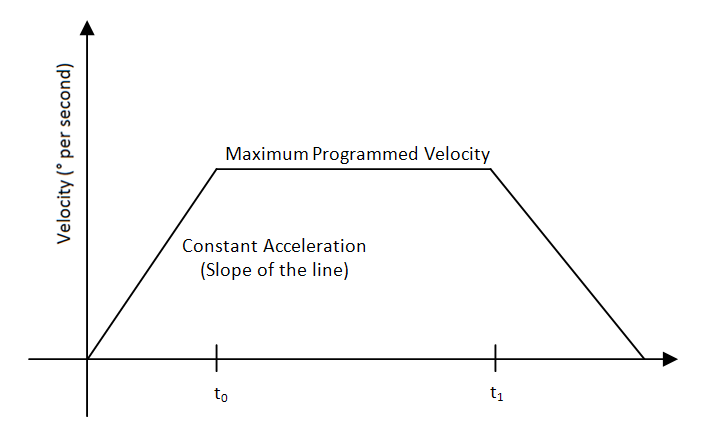
\includegraphics[scale=.3]{tmp.png}
	\end{figure}
	
	\tab The problem with TMP is the initial (infinitesimal) amount of acceleration required over the first instant to start the profile. This creates inconsistencies in following the profile as time increases. To fix this, the line used to accelerate to maximum velocity must be replaced with a function that has, ideally, infinite derivatives. One such function is sin.
	\tab The goal of this paper is to create a new motion profile that compensates for this inconsistency but is still efficient. The only constants defined by the user of SMP are $v_{max}$, $a_{max}$, and $D$, which are the maximum velocity, max acceleration, and distance of the profile of the robot at any time.
	
	\section{Sine Wave}
	\tab A sin wave can be modified from it's parent function in order to fit a certain domain and range. In it's most general form, the modified sin wave is defined by:
	\[sin(x) \rightarrow \frac{sin(kt - \frac{\pi}{2}) + 1}{c}, k = \frac{\pi}{x_{max}}, c = \frac{2}{y_{max}}\]
	\tab From the perspective of a motion profile, the maximum y value will be the maximum velocity ($y_{max} = t_{interval}$) and the maximum x value will be the time the profile takes to complete ($x_{max} = v_{max}$). Therefore, the new sin wave is defined as:
	\[velocity = v_{mod}(t) = \frac{sin(kt - \frac{\pi}{2}) + 1}{c}, c = \frac{2}{v_{max}}, k = \frac{\pi}{t_{interval}}\]
	\tab The derivative of velocity is acceleration, and thus the derivative of this function is:
	\[acceleration = a_{mod}(t) = \frac{k}{c} cos(kt - \frac{\pi}{2}), c = \frac{2}{v_{max}}, k = \frac{\pi}{t_{interval}}\]
	
	\section{Using the Modified Sin Wave}
	\tab The acceleration portion of the SMP can be visualized in this image:
	\begin{figure}[h]
		\centering
		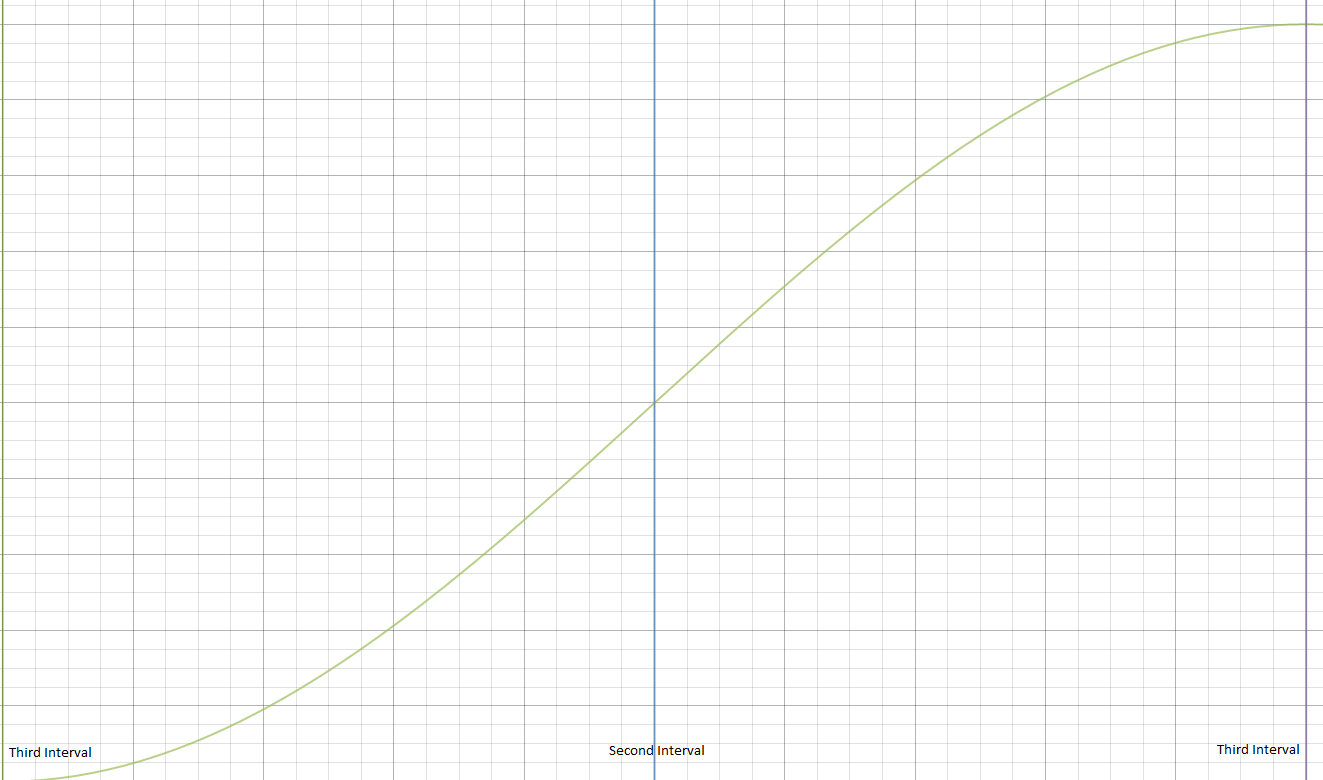
\includegraphics[scale=.3]{acceleration.png}
	\end{figure}
	
	\tab The equation for the velocity describes only the acceleration section of the SMP. The entire profile can be defined by the piecewise function defined below, which applies maximum velocity between the acceleration and deceleration intervals.
	\[v(t) = \begin{cases} 
	v_{mod}(t) & t < t_3  \\
	v_{max} & t_3 \leq t\leq t_4 \\
	-v_{mod}(t) & t > t_f
	\end{cases}\]
	\tab Using this piecewise function, the entire profile is shaped like the trapezoidal motion profile, but is much smoother and easier for a robot to follow.
	
	\chapter{Why It Works}
	\section{Problem with TMP}
	\tab 
	
	\chapter{Determining Time Intervals}
	\section{SMP Time Invervals}
	\tab The SMP graph is split into 6 important time intervals, referred to as $t_0...t_5$ and lastly $t_f$. The following table describes each interval.
	
	\begin{center}
		\begin{tabular}{| l | l |}
			\hline
			$t_1$ & the initial time of the SMP profile \\ \hline
			$t_2$ & the time at which the robot has the highest acceleration \\ \hline
			$t_3$ & the time at which the robot stops accelerating and is holding constant velocity \\ \hline
			$t_4$ & the time at which the robot starts decelerating \\ \hline
			$t_5$ & the time at which the robot has the highest deceleration \\ \hline
			$t_f$ & the final time of the profile (aka $t_profile$) \\ \hline
		\end{tabular}
	\end{center}
	
	\section{First Interval}
	\tab The initial time ($t_1$) of the profile can be found by grabbing time from the robot's FGPA. However, for the sake of calculating the intervals, the initial time will be 0.
	
	\section{Second and Third Interval}
	\tab The acceleration of the robot is highest at $t_2$, which can be proved by plugging in any numbers to the acceleration equation and determining the maximum of the function on the domain. $t_2 = \frac{t_3}{2}$ because the maximum acceleration occurs at the halfway point between 0 velocity and maximum velocity.
	
	\tab Mathematically, this can be represented by setting $t = t_2 = \frac{t_3}{2}$. Note that because the velocity equation is only defined for the interval between $t_1$ and $t_3$, $t_{end} = t_3$, and thus $c = \frac{2}{t_3}$. Plugging these values into $a_mod(t)$, we get the following derivation.
	\[a_{max} = \frac{k}{c} cos(\frac{t_3}{2} k - \frac{\pi}{2}), c = \frac{2}{v_{max}}, k = \frac{\pi}{t_{3}}\]
	\[a_{max} = \frac{\frac{\pi}{t_3}}{\frac{2}{v_{max}}} cos(\frac{\pi}{t_3} \frac{t_3}{2} - \frac{\pi}{2})\]
	\[a_{max} = \frac{v_{max}\pi}{2t_3} cos(\frac{\pi}{2} - \frac{\pi}{2})\]
	\[a_{max} = \frac{v_{max}\pi}{2t_3}\]
	\[t_3 = \frac{v_{max}\pi}{2a_{max}}\]
	\[t_2 = \frac{t_3}{2} = \frac{v_{max}\pi}{4a_{max}}\]
	
	\section{Fourth Interval}
	\tab We start with the assumption that the addition of the integral of the acceleration and deceleration portions plus the integral of the constant velocity portion results in the total distance that the profile travels. This is represented by:
	\[D = 2\int_{t_1}^{t_3}v_{mod}(t)dt + \int_{t_3}^{t_4}v_{max}dt\]
	\tab This can be simplified through the following derivation, to an equation for the third and fourth intervals.
	\[D = 2\int_{t_1}^{t_3}v_{mod}(t)dt + v_{max}(t_4 - t_3)\]
	\[D = 2\int_{t_1}^{t_3}\frac{sin(kt - \frac{\pi}{2}) + 1}{c}dt + v_{max}(t_4 - t_3)\]
	\[D = 2\left[\int_{t_1}^{t_3}\frac{sin(kt - \frac{\pi}{2})}{c}dt + \int_{t_1}^{t_3}\frac{1}{c}dt\right] + v_{max}(t_4 - t_3)\]
	\[D = 2\left[\int_{t_1}^{t_3}\frac{sin(kt - \frac{\pi}{2})}{c}dt + \frac{t_3 - t_1}{c}\right] + v_{max}(t_4 - t_3)\]
	\[substitution \rightarrow u = kt - \frac{\pi}{2}, du = kdt, \frac{1}{k}du = dt\]
	\[D = 2\left[-\frac{1}{ck}\left[cos(kt - \frac{\pi}{2})\right]_{t_1}^{t_3} + \frac{t_3 - t_1}{c}\right] + v_{max}(t_4 - t_3)\]
	\[D = 2\left[-\frac{1}{ck}\left[cos(kt_3 - \frac{\pi}{2}) - cos(kt_1 - \frac{\pi}{2})\right] + \frac{t_3 - t_1}{c}\right] + v_{max}(t_4 - t_3)\]
	\tab From here, $t_1$ is the beginning of the profile and can be set to 0 for the rest of this derivation.
	\[D = 2\left[-\frac{1}{ck}cos(kt_3 - \frac{\pi}{2}) + \frac{t_3}{c}\right] + v_{max}(t_4 - t_3)\]
	\tab Finally, we must plug in $k = \frac{\pi}{t_3}$ and $c = \frac{2}{v_{max}}$.
	\[D = 2\left[-\frac{t_3v_{max}}{2\pi}cos(\frac{\pi}{2}) + \frac{t_3v_{max}}{2}\right] + v_{max}(t_4 - t_3)\]
	\[D = 2(\frac{t_3v_{max}}{2}) + v_{max}(t_4 - t_3)\]
	\[D = t_3v_{max} + v_{max}(t_4 - t_3)\]
	\[D = v_{max}(t_3 + t_4 - t_3)\]
	\[t_4 = \frac{D}{v_{max}}\]
	
	\section{Final Interval}
	\tab The total time of the profile, $t_f$, can be easily defined using symmetry. The acceleration and deceleration portions are exactly equal, which means $t_f = 2t_3 + (t_4 - t_3) = t_4 + t_3$.
	\[t_f = t_4 + t_3\]
	\[t_f = \frac{D}{v_{max}} + \frac{v_{max}\pi}{2a_{max}}\]
	\[t_f = \frac{2a_{max}D}{2a_{max}v_{max}} + \frac{(v_{max})^2\pi}{2v_{max}a_{max}}\]
	\[t_f = \frac{2a_{max}D + (v_{max})^2\pi}{2a_{max}v_{max}}\]
	
	\section{Fifth Interval}
	\tab The fifth interval is easily defined by the equation $t_f - t_5 = t_2$, or $t_5 = t_f - t_2$. This requires that $t_f$ is defined.
	\[t_5 = t_f - t_2\]
	\[t_5 = \frac{2a_{max}D + (v_{max})^2\pi}{2a_{max}v_{max}} - \frac{v_{max}\pi}{4a_{max}}\]
	\[t_5 = \frac{4a_{max}D + (v_{max})^2\pi}{4a_{max}v_{max}}\]
	
	\chapter{Time Interval Calculation Alternatives}
	\section{Second Interval Alt}
	\section{Fifth Interval Alt}
	
\end{document}